\documentclass{article}
\usepackage{float}
\usepackage{graphicx}
\usepackage{fancyhdr}

\usepackage{geometry}
\geometry{margin=1in}
\setlength{\headheight}{49.4pt}
\pagestyle{fancy}
\fancyhf{}
\rhead{
    \centering
  \begin{tabular*}{\textwidth}{@{\extracolsep{\fill}}ccc}
    \small University of Florida & \textbf{\small EEL3111C - Circuits} & \small Rottenberg, Cole Harrison\\
    \small Electrical \& Computer Engineering Dept. & \small Lab 8: Diode Applications & \small Class \#: 20931 \\
    \small Page \thepage & \small Revision: 0 & \small \today \\
  \end{tabular*}
}

\begin{document}
% I need a bold horizontal line

\begin{center}
    \hrule
    \vspace{0.2cm}
    \textbf{\large REQUIREMENTS NOT MET}
    \vspace{0.2cm}
    \hrule
\end{center}
% Bullet points on what was not met
\begin{itemize}
    \item \textbf{Requirement 1:} The requirement was not met because of this reason.
    \item \textbf{Requirement 2:} The requirement was not met because of this reason.
    \item \textbf{Requirement 3:} The requirement was not met because of this reason.
\end{itemize}

\begin{center}
    \hrule
    \vspace{0.2cm}
    \textbf{\large PROBLEMS ENCOUNTERED}
    \vspace{0.2cm}
    \hrule
\end{center}
% More Bullet points with filler text
\begin{itemize}
    \item \textbf{Problem 1:} The problem was encountered because of this reason.
    \item \textbf{Problem 2:} The problem was encountered because of this reason.
    \item \textbf{Problem 3:} The problem was encountered because of this reason.
\end{itemize}

\begin{center}
    \hrule
    \vspace{0.2cm}
    \textbf{\large INTRODUCTION}
    \vspace{0.2cm}
    \hrule
\end{center}

Now we start our introduction to our write up
For your write up, write a brief introduction to what you are doing in the in lab. two to four sentences. 
Omit this section for the prelab.


\begin{center}
    \hrule
    \vspace{0.2cm}
    \textbf{\large DISCUSSION}
    % A horizontal line here
    \vspace{0.2cm}
    \hrule
\end{center}

\textbf{\large8.5 Pre-Lab Requirements:}

\textbf{8.5.1 LTspice Simulations:}
\begin{enumerate}
    \item Set the input to a 1 kHz, 5 V amplitude
sine wave and run a transient simulation with a stop time of 1m (.tran 1m)
and plot the input and output. To use the 1N4148 diode model, right click on
the diode after placing it, Pick New Diode, and then choose the 1N4148 model
(Mfg. OnSemi). Save an image of the circuit and the plot of the input and
output voltage for submission to canvas.
    \begin{figure}[H]
        \centering
        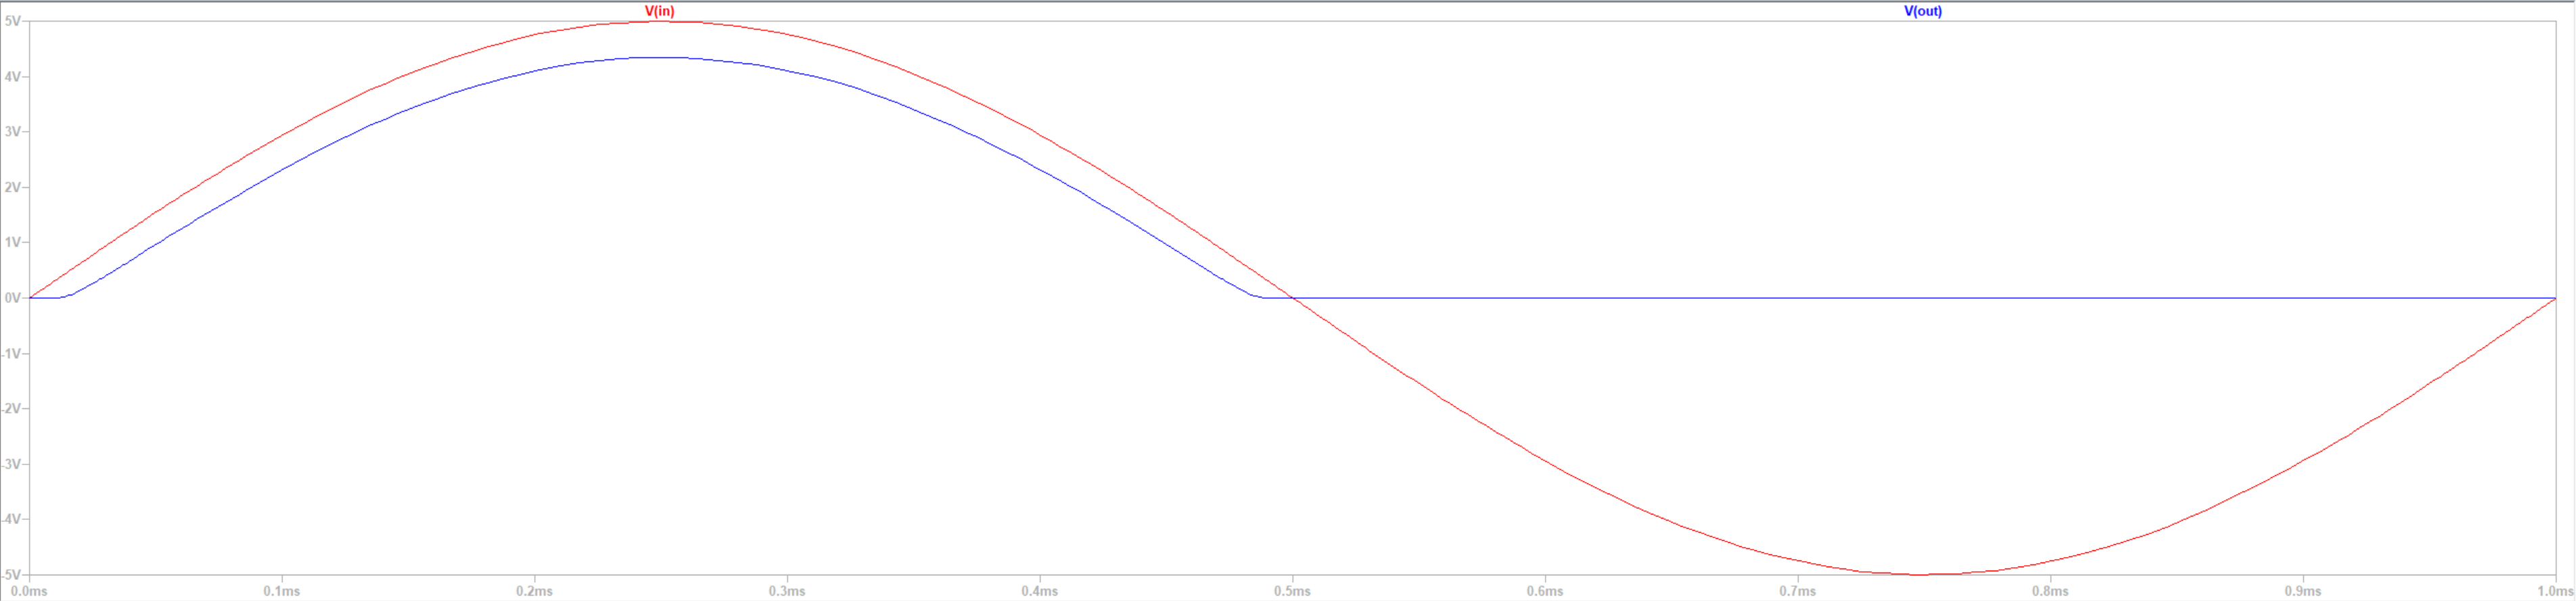
\includegraphics[width=0.75\textwidth]{fig8_2_a.png}
        \caption{HALF WAVE RECTIFIER PLOT} 
        \label{fig:half_wave_rectifier}
    \end{figure}
    \begin{figure}[H]
        \centering
        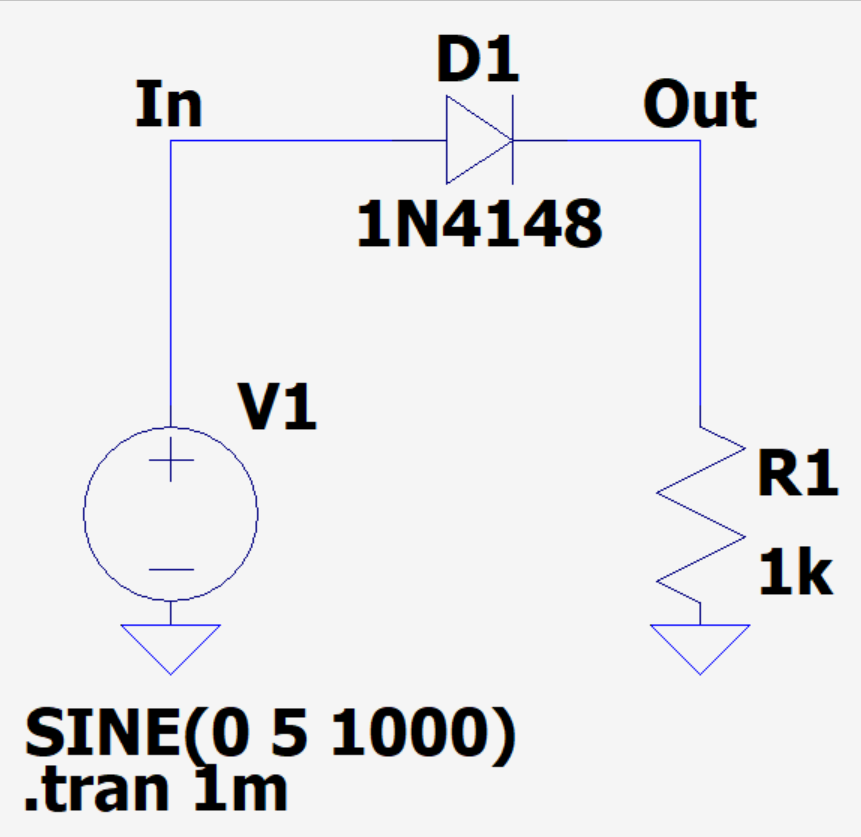
\includegraphics[width=0.75\textwidth]{circuit8_2_a.png}
        \caption{HALF WAVE RECTIFIER CIRCUIT} 
        \label{fig:half_wave_rectifier_circuit}
    \end{figure}
    \item Build the circuit in Figure 8.3 (a). Set the input to a 100 kHz, 5 V amplitude
sine wave and run a transient simulation with a stop time of 50u (.tran 50u)
and step through possible capacitor values using the following spice directive:
    \begin{figure}[H]
        \centering
        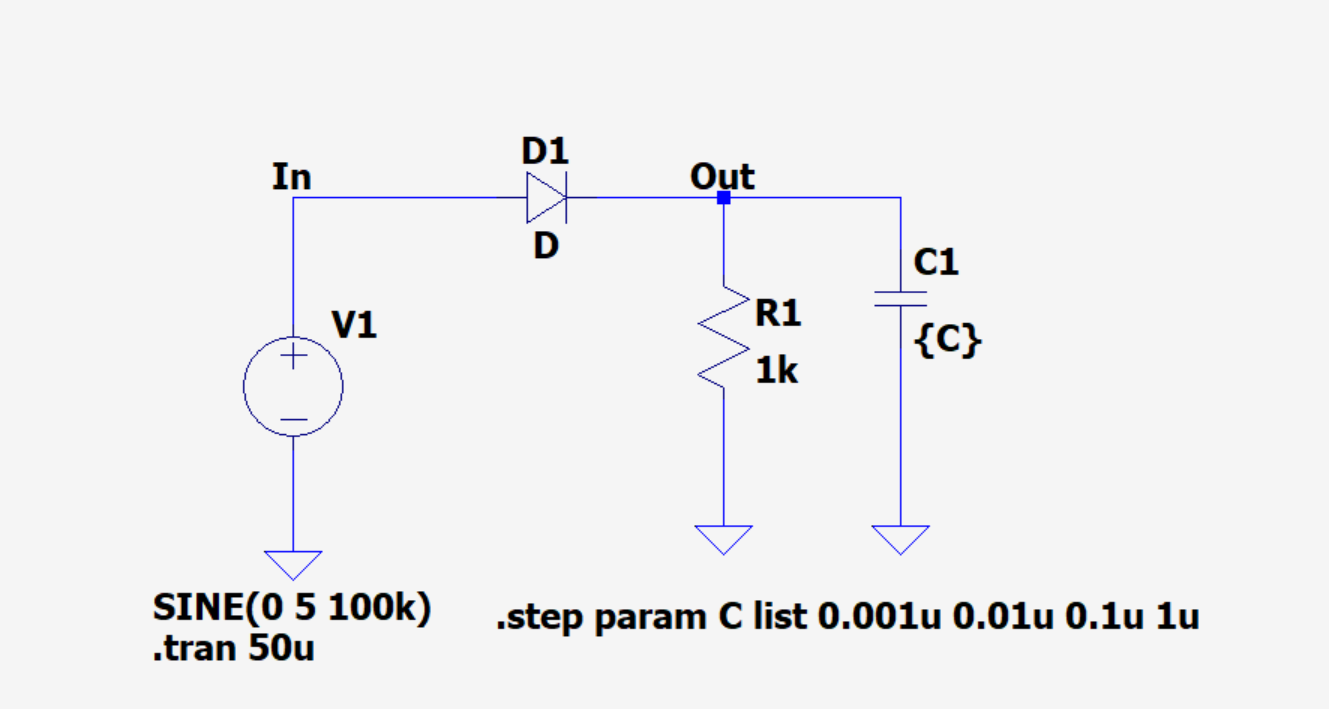
\includegraphics[width=0.75\textwidth]{circuit8_3a.png}
        \caption{HALF WAVE RECTIFIER CIRCUIT WITH  CAPACITOR} 
        \label{fig:HALF WAVE RECTIFIER CIRCUIT WITH CAPACITOR}
    \end{figure}

    \begin{figure}[H]
        \centering
        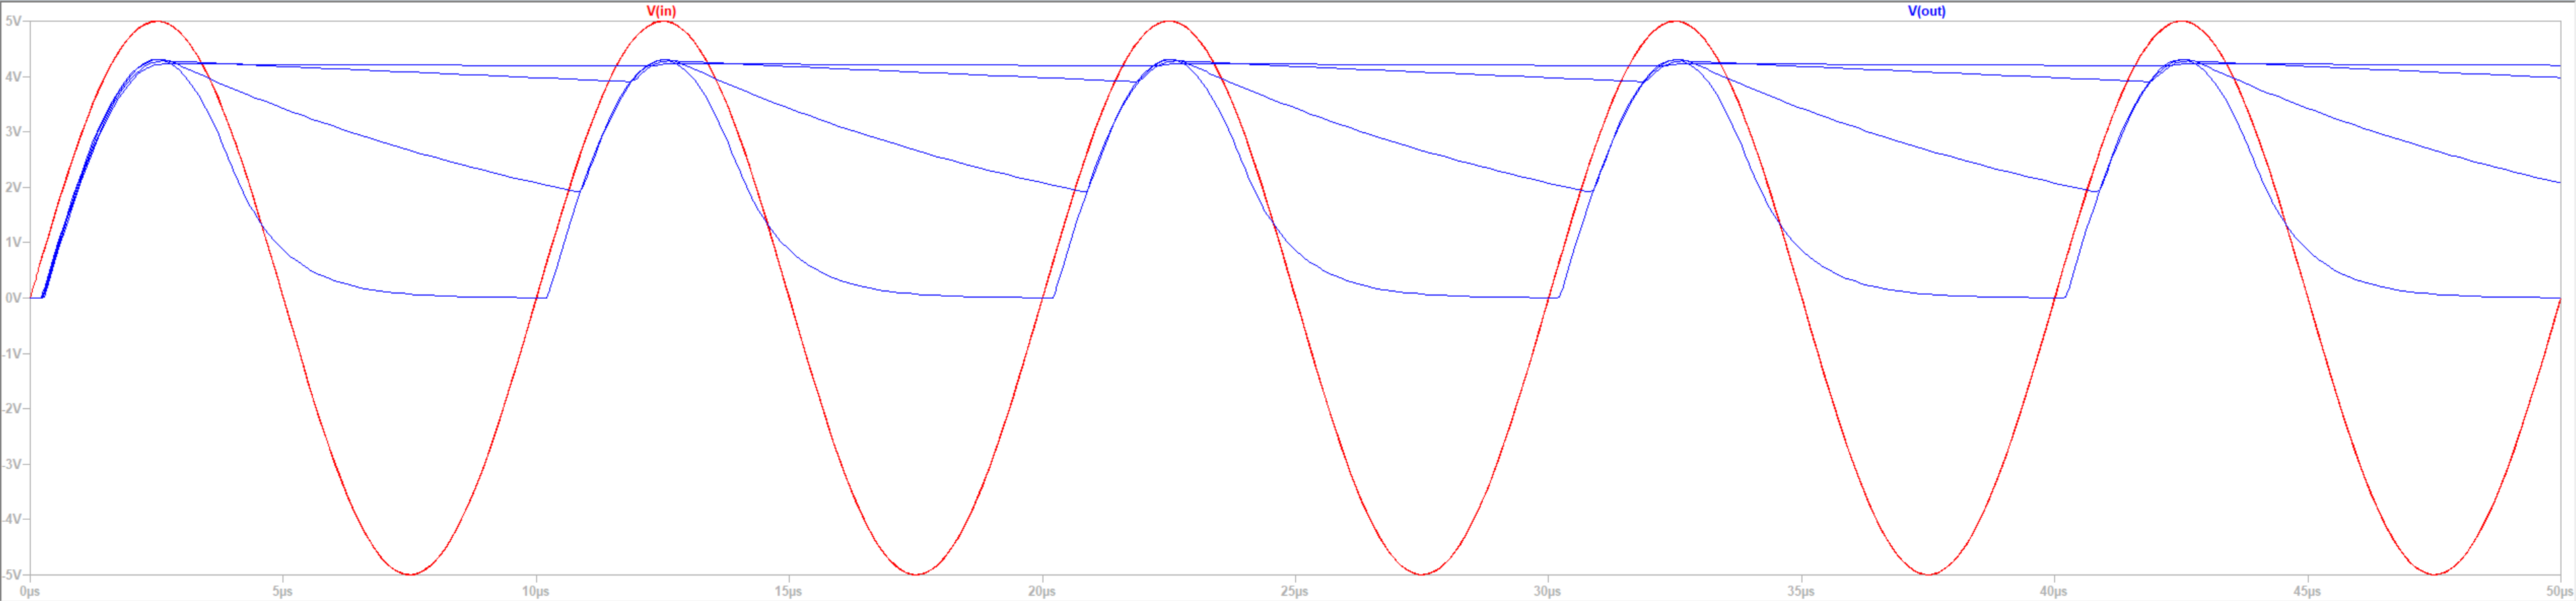
\includegraphics[width=0.75\textwidth]{plot8_3a.png}
        \caption{HALF WAVE RECTIFIER CIRCUIT WITH CAPACITOR PLOT}
        \label{fig:half_wave_rectifier_plot}
    \end{figure}
    \item Build the circuit in Figure 8.4. Use the default LED model in LTSpice, and
download "slcj016.zip" file from Canvas "Lab Related Files" folder for the LM393
comparator model. Don’t use the "slcj016b.zip" for the comparator model from 
TI because it’s a newer model that doesn’t work for input higher than (Vcc-2V).
Power the LM393 with +/-5 V. Set the input voltage to a 1 kHz, 5 V amplitude
sine wave and run a transient solution with a stop time of 2m (.tran 2m). Plot
the input voltage and the current through each diode. Save an image of the
circuit and the plot for submission to canvas
    \begin{figure}[H]
        \centering
        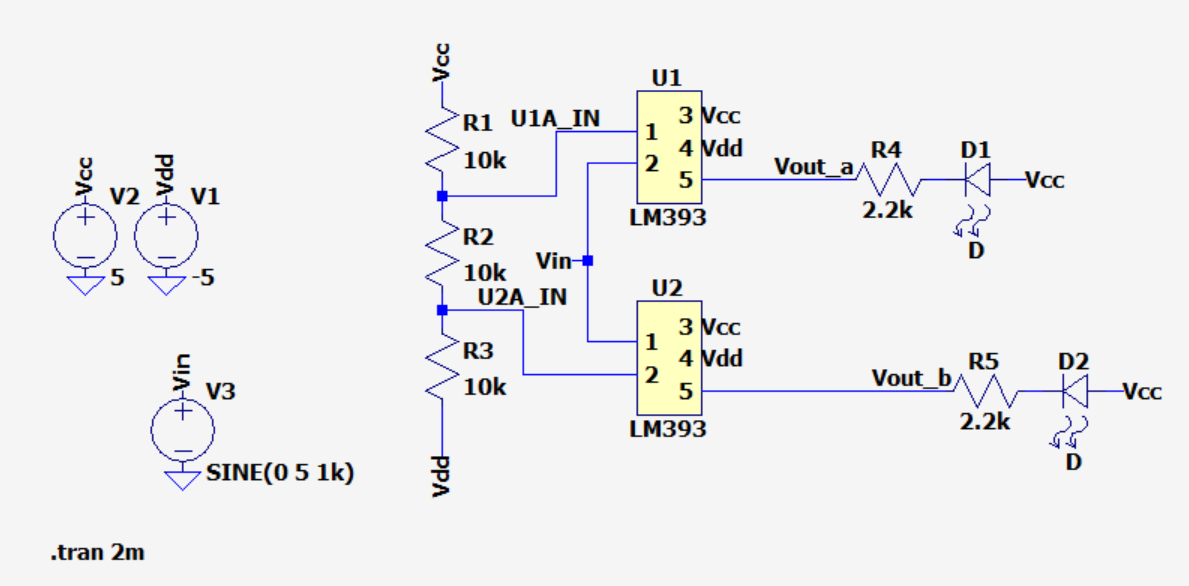
\includegraphics[width=0.75\textwidth]{circuit8_4.png}
        \caption{COMPARATOR CIRCUIT} 
        \label{fig:comp-circuit}
    \end{figure}

    \begin{figure}[H]
        \centering
        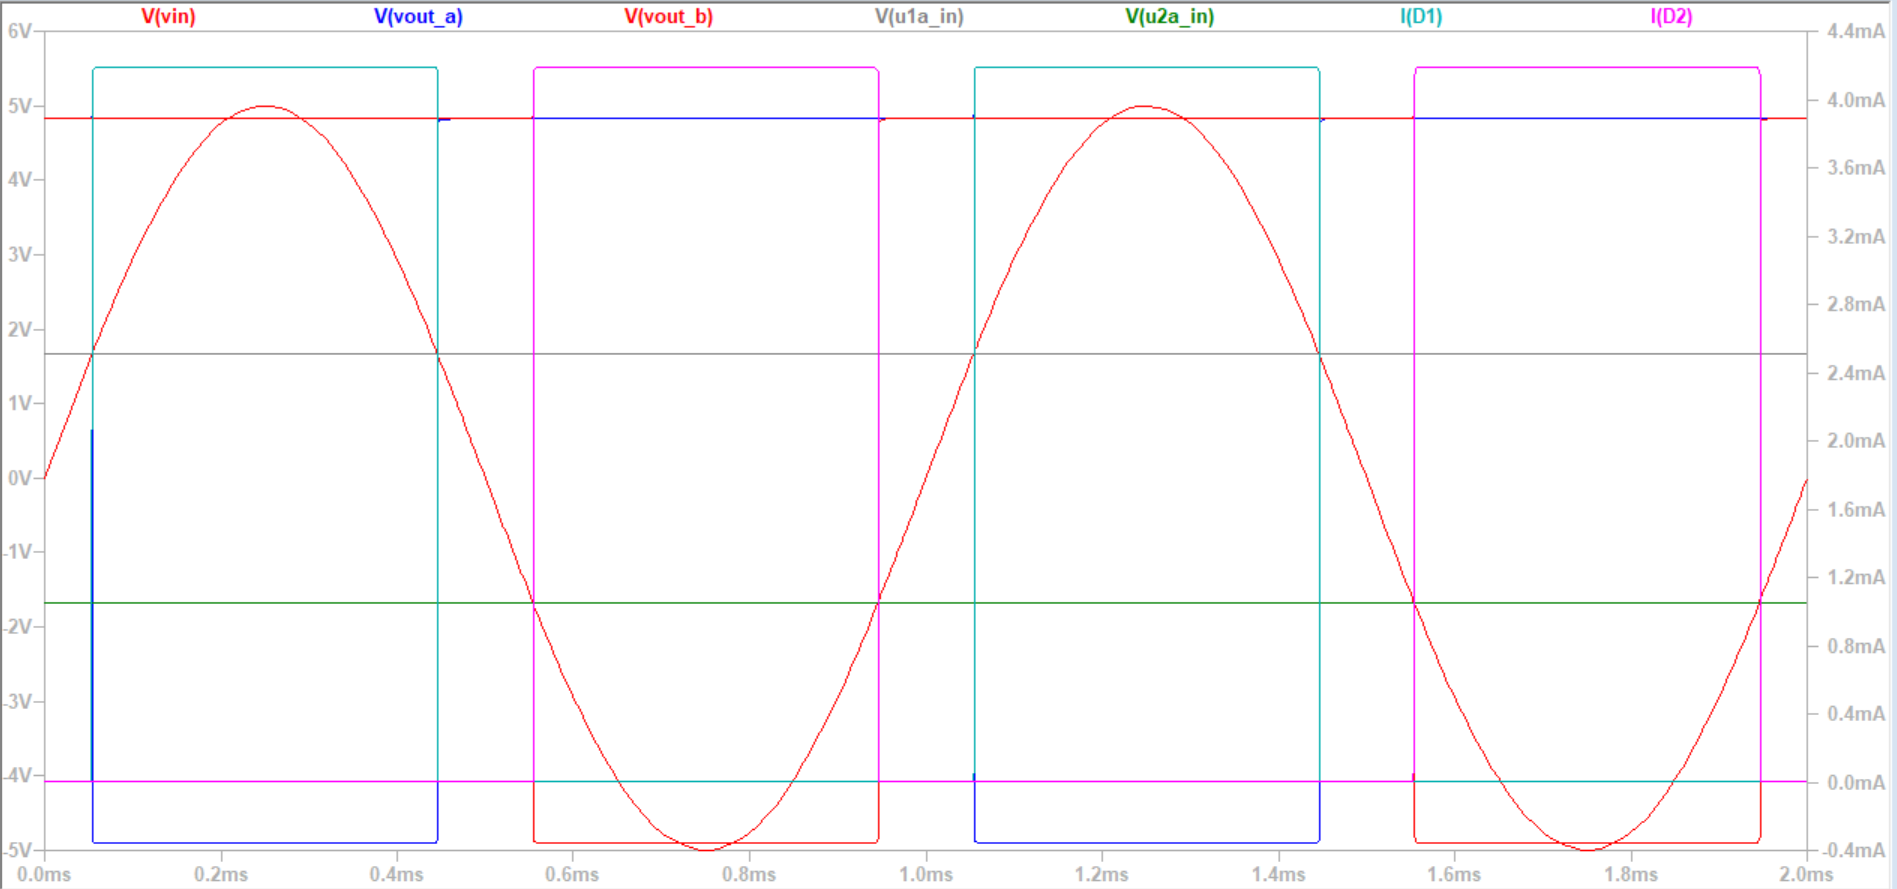
\includegraphics[width=0.75\textwidth]{plot8_4.png}
        \caption{COMPARATOR PLOT} 
        \label{fig:comp-plot}
    \end{figure}
    \item Build the circuit in Figure 8.7. Power the LM393 and TLV272 with +/-5 V.
Set the input voltage to a 1kHz, 0.1 V amplitude sine wave and run a transient
solution with a stop time of 2m. Choose the value for R1, 10k pot, so that
the diodes conduct current and illuminate. Plot the input voltage, output of
the op amp, positive and negative inputs to the comparator, and the current
through both LEDs. (6 items total). Save an image of the circuit and the plot
for submission to canvas.
    \begin{figure}[H]
        \centering
        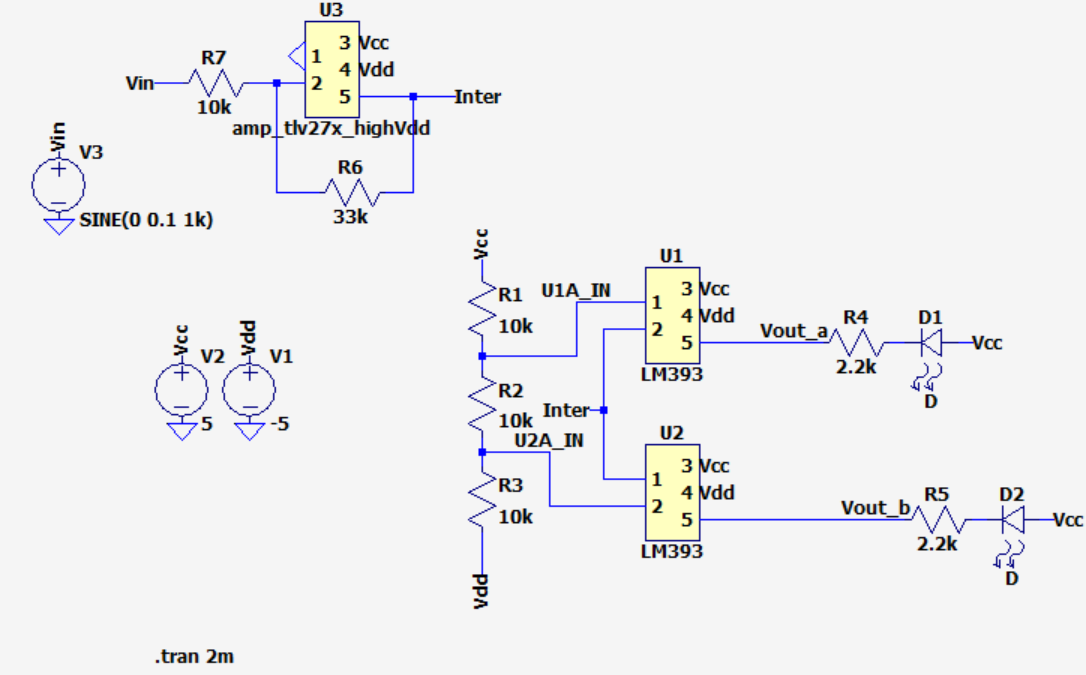
\includegraphics[width=0.75\textwidth]{circuit8_7.png}
        \caption{COMPARATOR CIRCUIT WITH OP-AMP} 
        \label{fig:comp-circuit-op-amp}
    \end{figure}

    \begin{figure}[H]
        \centering
        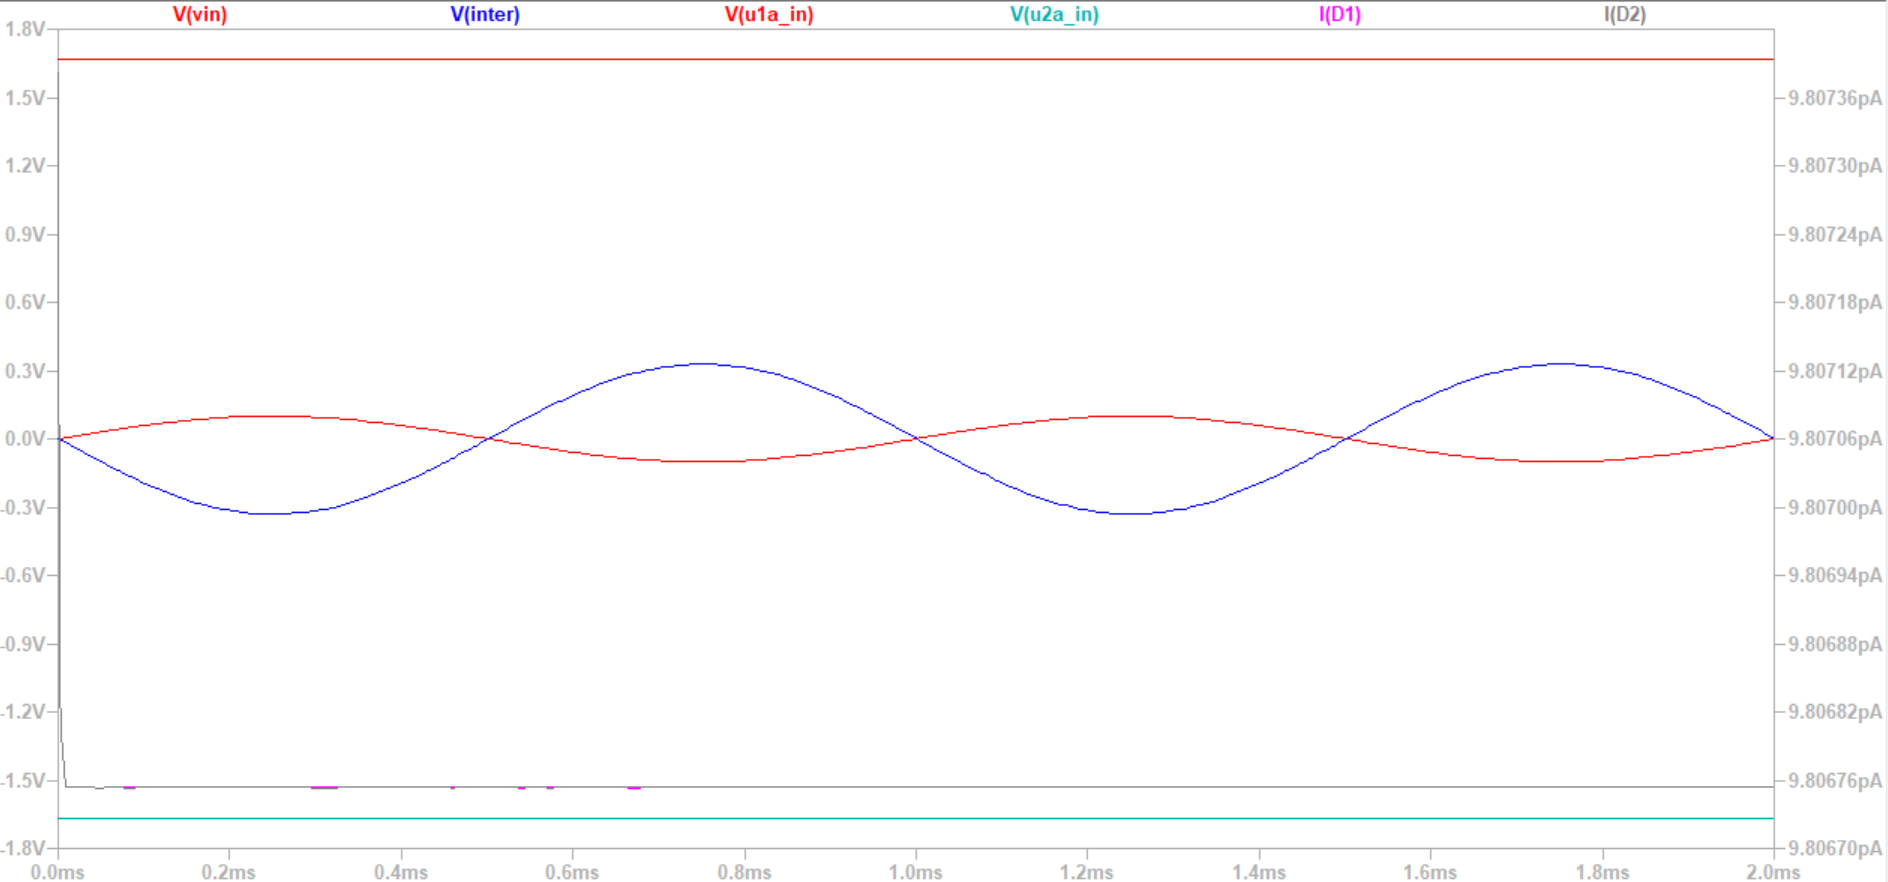
\includegraphics[width=0.75\textwidth]{plot8_7.png}
        \caption{COMPARATOR PLOT WITH OP-AMP} 
        \label{fig:comp-plot-op-amp}
    \end{figure}
\end{enumerate}
\textbf{8.5.2 Breadboard Implementation:}
\begin{enumerate}
    \item Build the circuit in Figure 8.4 on the breadboard. Use the LM393.
\end{enumerate}
\pagebreak
\begin{center}
    \hrule
    \vspace{0.2cm}
    \textbf{\large CONCLUSION}
    % A horizontal line here
    \vspace{0.2cm}
    \hrule
\end{center}

This is where I start to answer the questions in the lab. We only need to do this for the write up.

\end{document}